\chapter{Planos}

Este capítulo presenta la documentación gráfica del sistema de cableado estructurado de la Escuela Profesional de Enfermería de la UNSAAC. Los planos muestran la distribución de la red, los puntos de datos, canalizaciones, backbone, puesta a tierra y cobertura inalámbrica, y constituyen la guía técnica para la implementación, administración y mantenimiento del sistema.

\section{Plano de Ubicación General de la Red}
\label{sec:plano_ubicacion}

El plano de ubicación identifica la posición del edificio de Enfermería dentro del campus de la UNSAAC y su integración con la red institucional administrada por la DTIC. Para efectos del diseño, el edificio se conecta a la red de campus mediante fibra óptica tendida en canalización subterránea, conforme a la norma \mbox{ANSI/TIA-568-C.0}.

\begin{figure}[H]
    \centering
    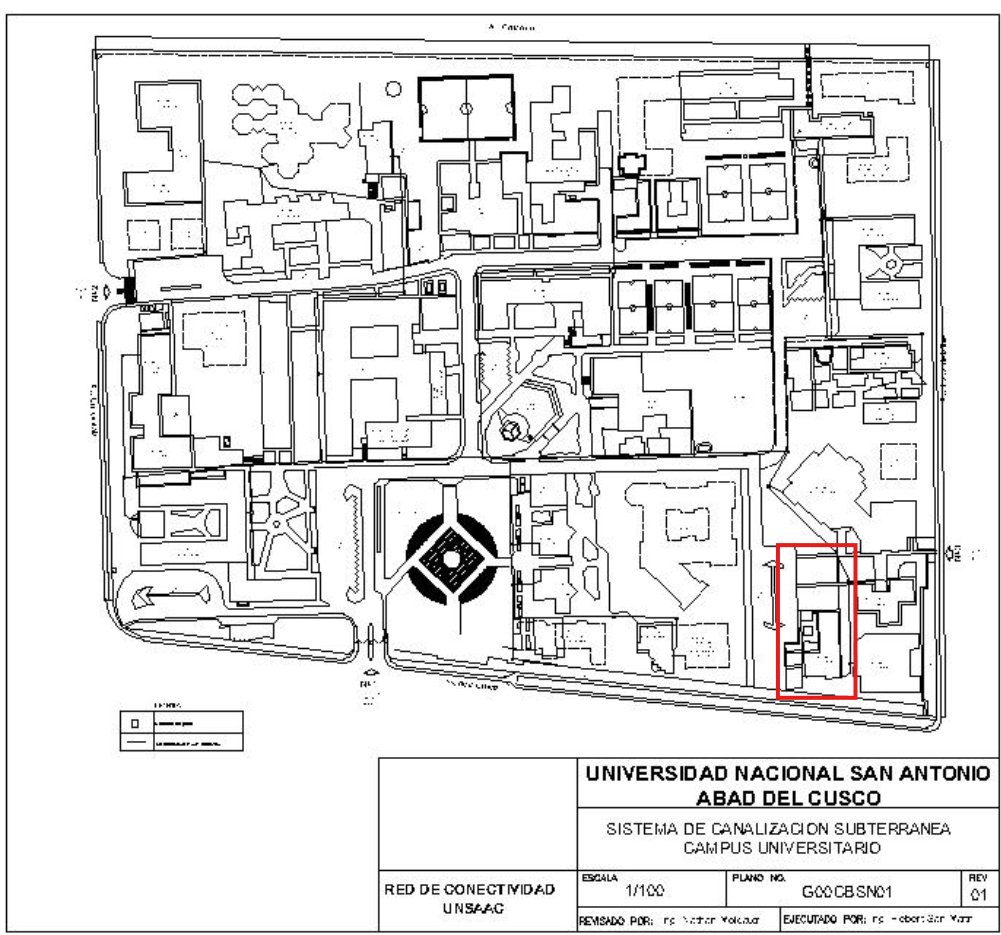
\includegraphics[width=0.92\textwidth]{images/imagenes/plano_campus.png}
    \caption{Plano de ubicación general — Campus UNSAAC. El edificio de la Escuela Profesional de Enfermería (Gabinete G09) se indica con el recuadro rojo en el sector sureste. Plano N.$^\circ$ G00CBSN01, Esc.\ 1:100.}
    \label{fig:plano_ubicacion_campus}
\end{figure}

\section{Planos de Planta con Puntos de Red y Canalizaciones}
\label{sec:planos_planta}

Los planos de planta muestran la ubicación exacta de cada punto de red (outlet de telecomunicaciones), las rutas de canalización y el recorrido del cableado horizontal por nivel. Para su elaboración se realizó visita técnica al edificio, inventario de ambientes con demanda de conectividad según \mbox{ANSI/TIA-568-C.1}, análisis de infraestructura existente y digitalización en AutoCAD sobre los planos arquitectónicos originales.

\subsection{Sistema de Codificación de Puntos de Red}
Para la administración de la infraestructura física según la norma ANSI/TIA-606-B, cada enlace pasivo será etiquetado de manera idéntica en el conector del usuario (Faceplate) y en el panel de parcheo (Patch Panel) del Rack G09.
Se establece una nomenclatura alfanumérica estructurada bajo el formato \textbf{G09-N[X]-[Tipo][YY]}, enfocada puramente en datos, soporte inalámbrico y video vigilancia:

\begin{table}[H]
\centering
\caption{Estructura de etiquetado normativo para la capa física.}
\small
\begin{tabular}{ccp{8.5cm}}
\hline
\textbf{Componente} & \textbf{Identificador} & \textbf{Descripción Técnica} \\
\hline
\textbf{Gabinete Central} & G09 & Identifica al Rack Principal ubicado en el Piso 2. \\
\textbf{Nivel Físico} & N1 / N2 / N3 / N4 & Especifica el piso del edificio donde se encuentra el punto. \\
\textbf{Tipo de Nodo} & D / W / C & \textbf{D:} Punto de Datos fijo en pared (PC de escritorio). \newline \textbf{W:} Punto de Datos en techo para Access Point (Wi-Fi). \newline \textbf{C:} Punto de Datos aéreo para cámara de seguridad (CCTV). \\
\textbf{Correlativo} & 01, 02, 03\dots & Numeración secuencial de los puntos por tipo en cada piso. \\
\hline
\end{tabular}
\end{table}

\begin{figure}[H]
    \centering
    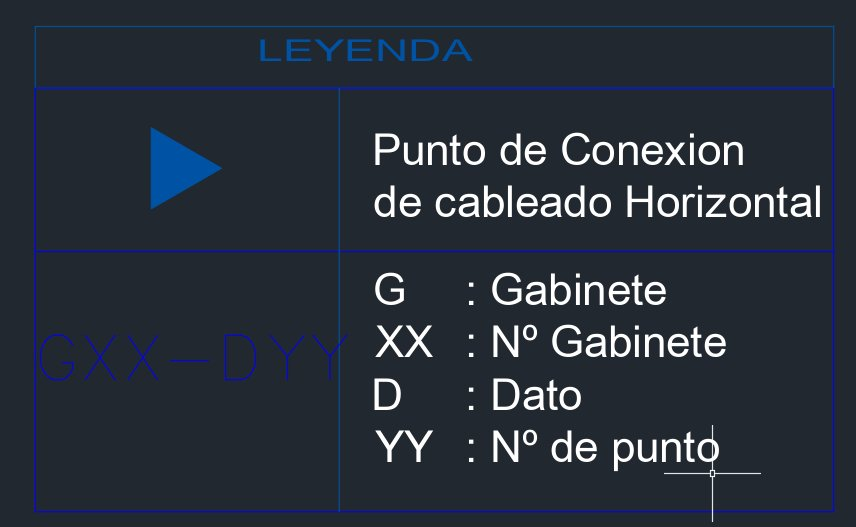
\includegraphics[width=0.70\textwidth]{images/imagenes/leyenda_puntos_red.png}
    \caption{Leyenda de simbología empleada en los planos de planta (puntos de red, canalizaciones y equipos).}
    \label{fig:leyenda_puntos}
\end{figure}

\subsection{Primer Nivel}
\begin{figure}[H]
    \centering
    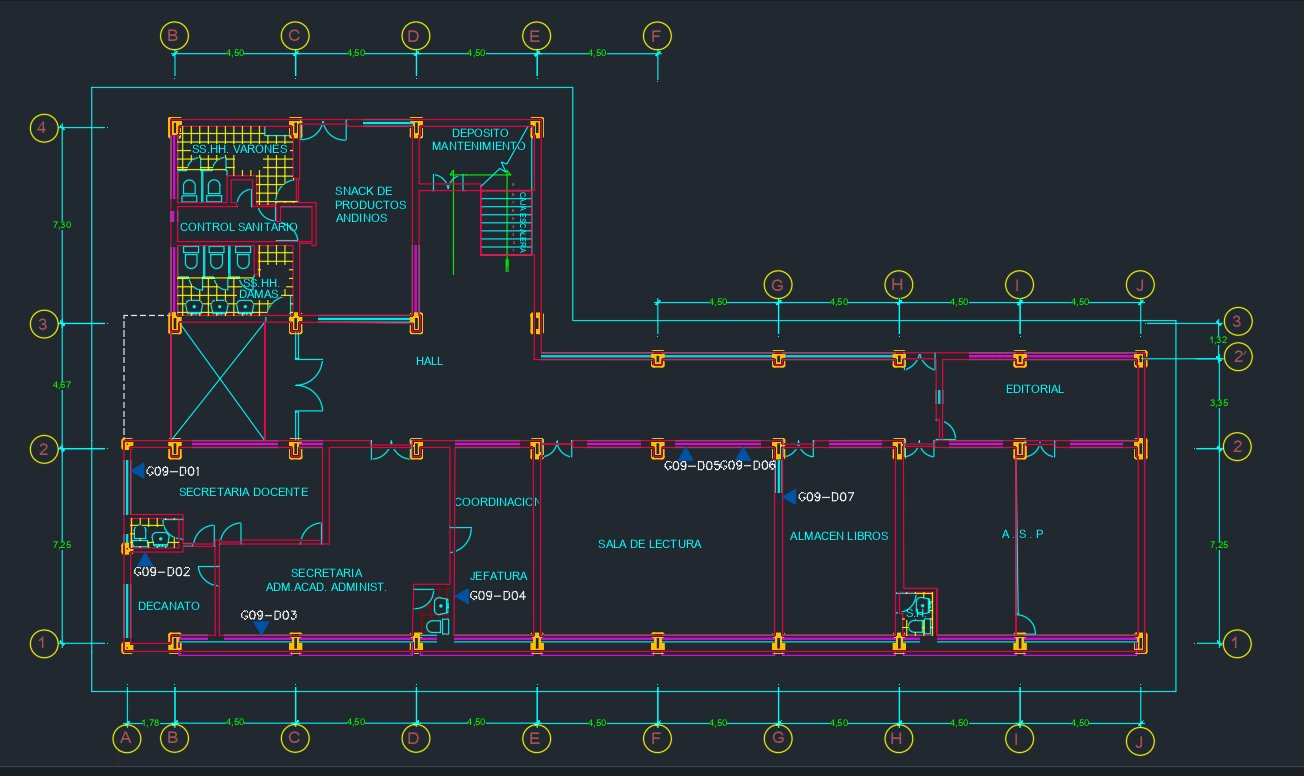
\includegraphics[width=0.97\textwidth]{images/imagenes/plano_primer_nivel.png}
    \caption{Plano del primer nivel con puntos de red G09-D01 a G09-D07 y rutas de canalización. Esc.\ 1:100.}
    \label{fig:plano_primer_nivel}
\end{figure}

\subsection{Segundo Nivel}
\begin{figure}[H]
    \centering
    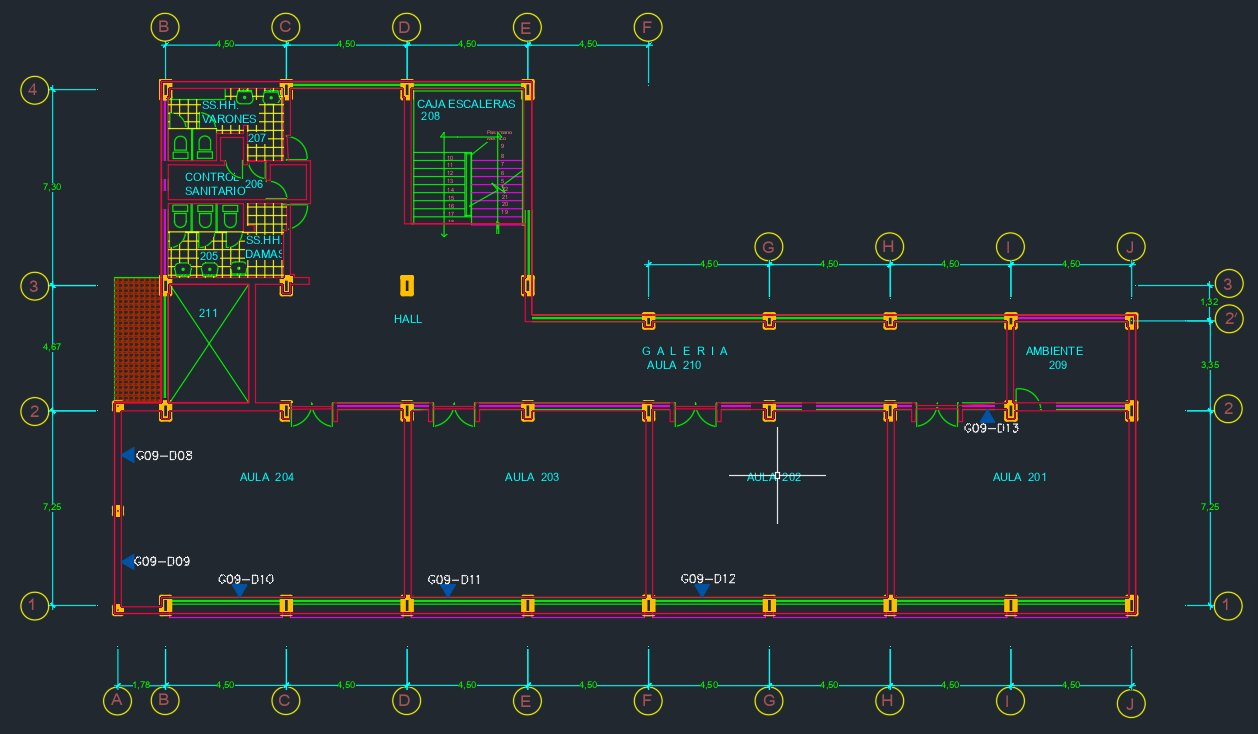
\includegraphics[width=0.97\textwidth]{images/imagenes/plano_segundo_nivel.png}
    \caption{Plano del segundo nivel con puntos de red G09-D08 a G09-D13 y rutas de canalización. Esc.\ 1:100.}
    \label{fig:plano_segundo_nivel}
\end{figure}

\subsection{Tercer Nivel}
\begin{figure}[H]
    \centering
    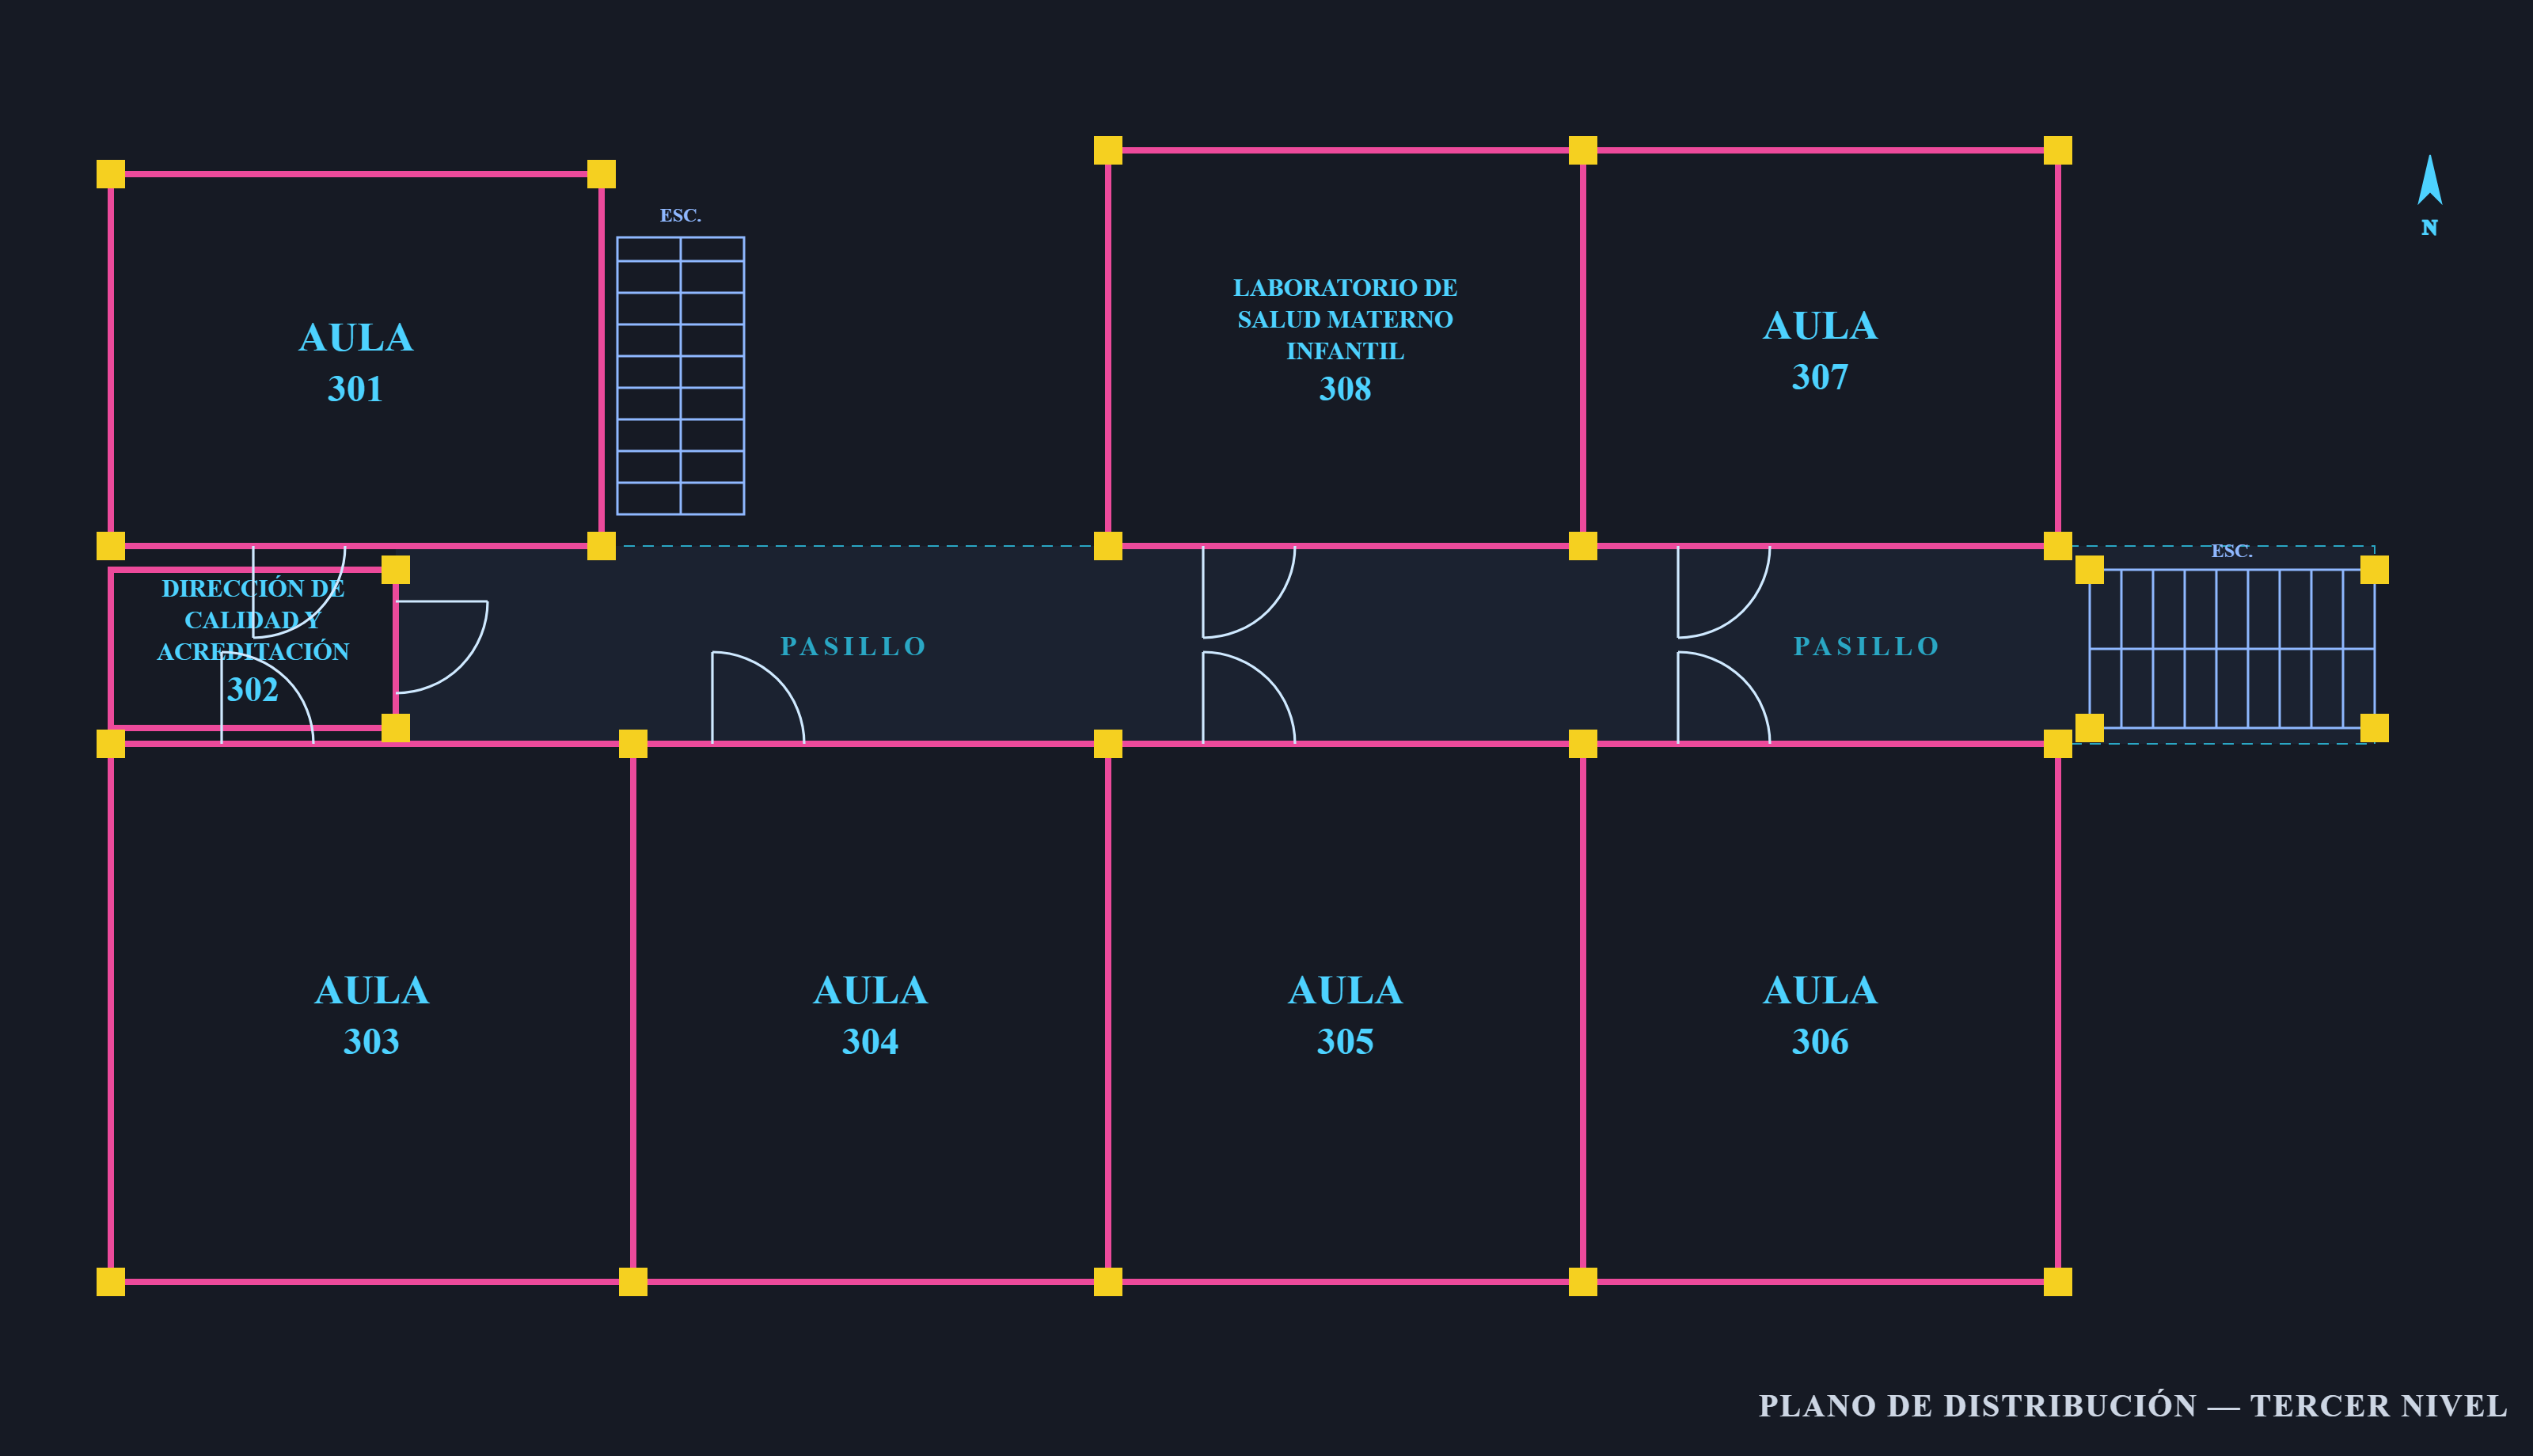
\includegraphics[width=0.97\textwidth]{images/imagenes/plano_tercer_nivel.png}
    \caption{Plano arquitectónico del tercer piso que detalla el recorrido de las rutas de distribución y las cajas de salida para los escritorios de los docentes en las aulas y laboratorios de simulación clínica.}
    \label{fig:plano_tercer_nivel}
\end{figure}

\subsection{Cuarto Nivel}
\begin{figure}[H]
    \centering
    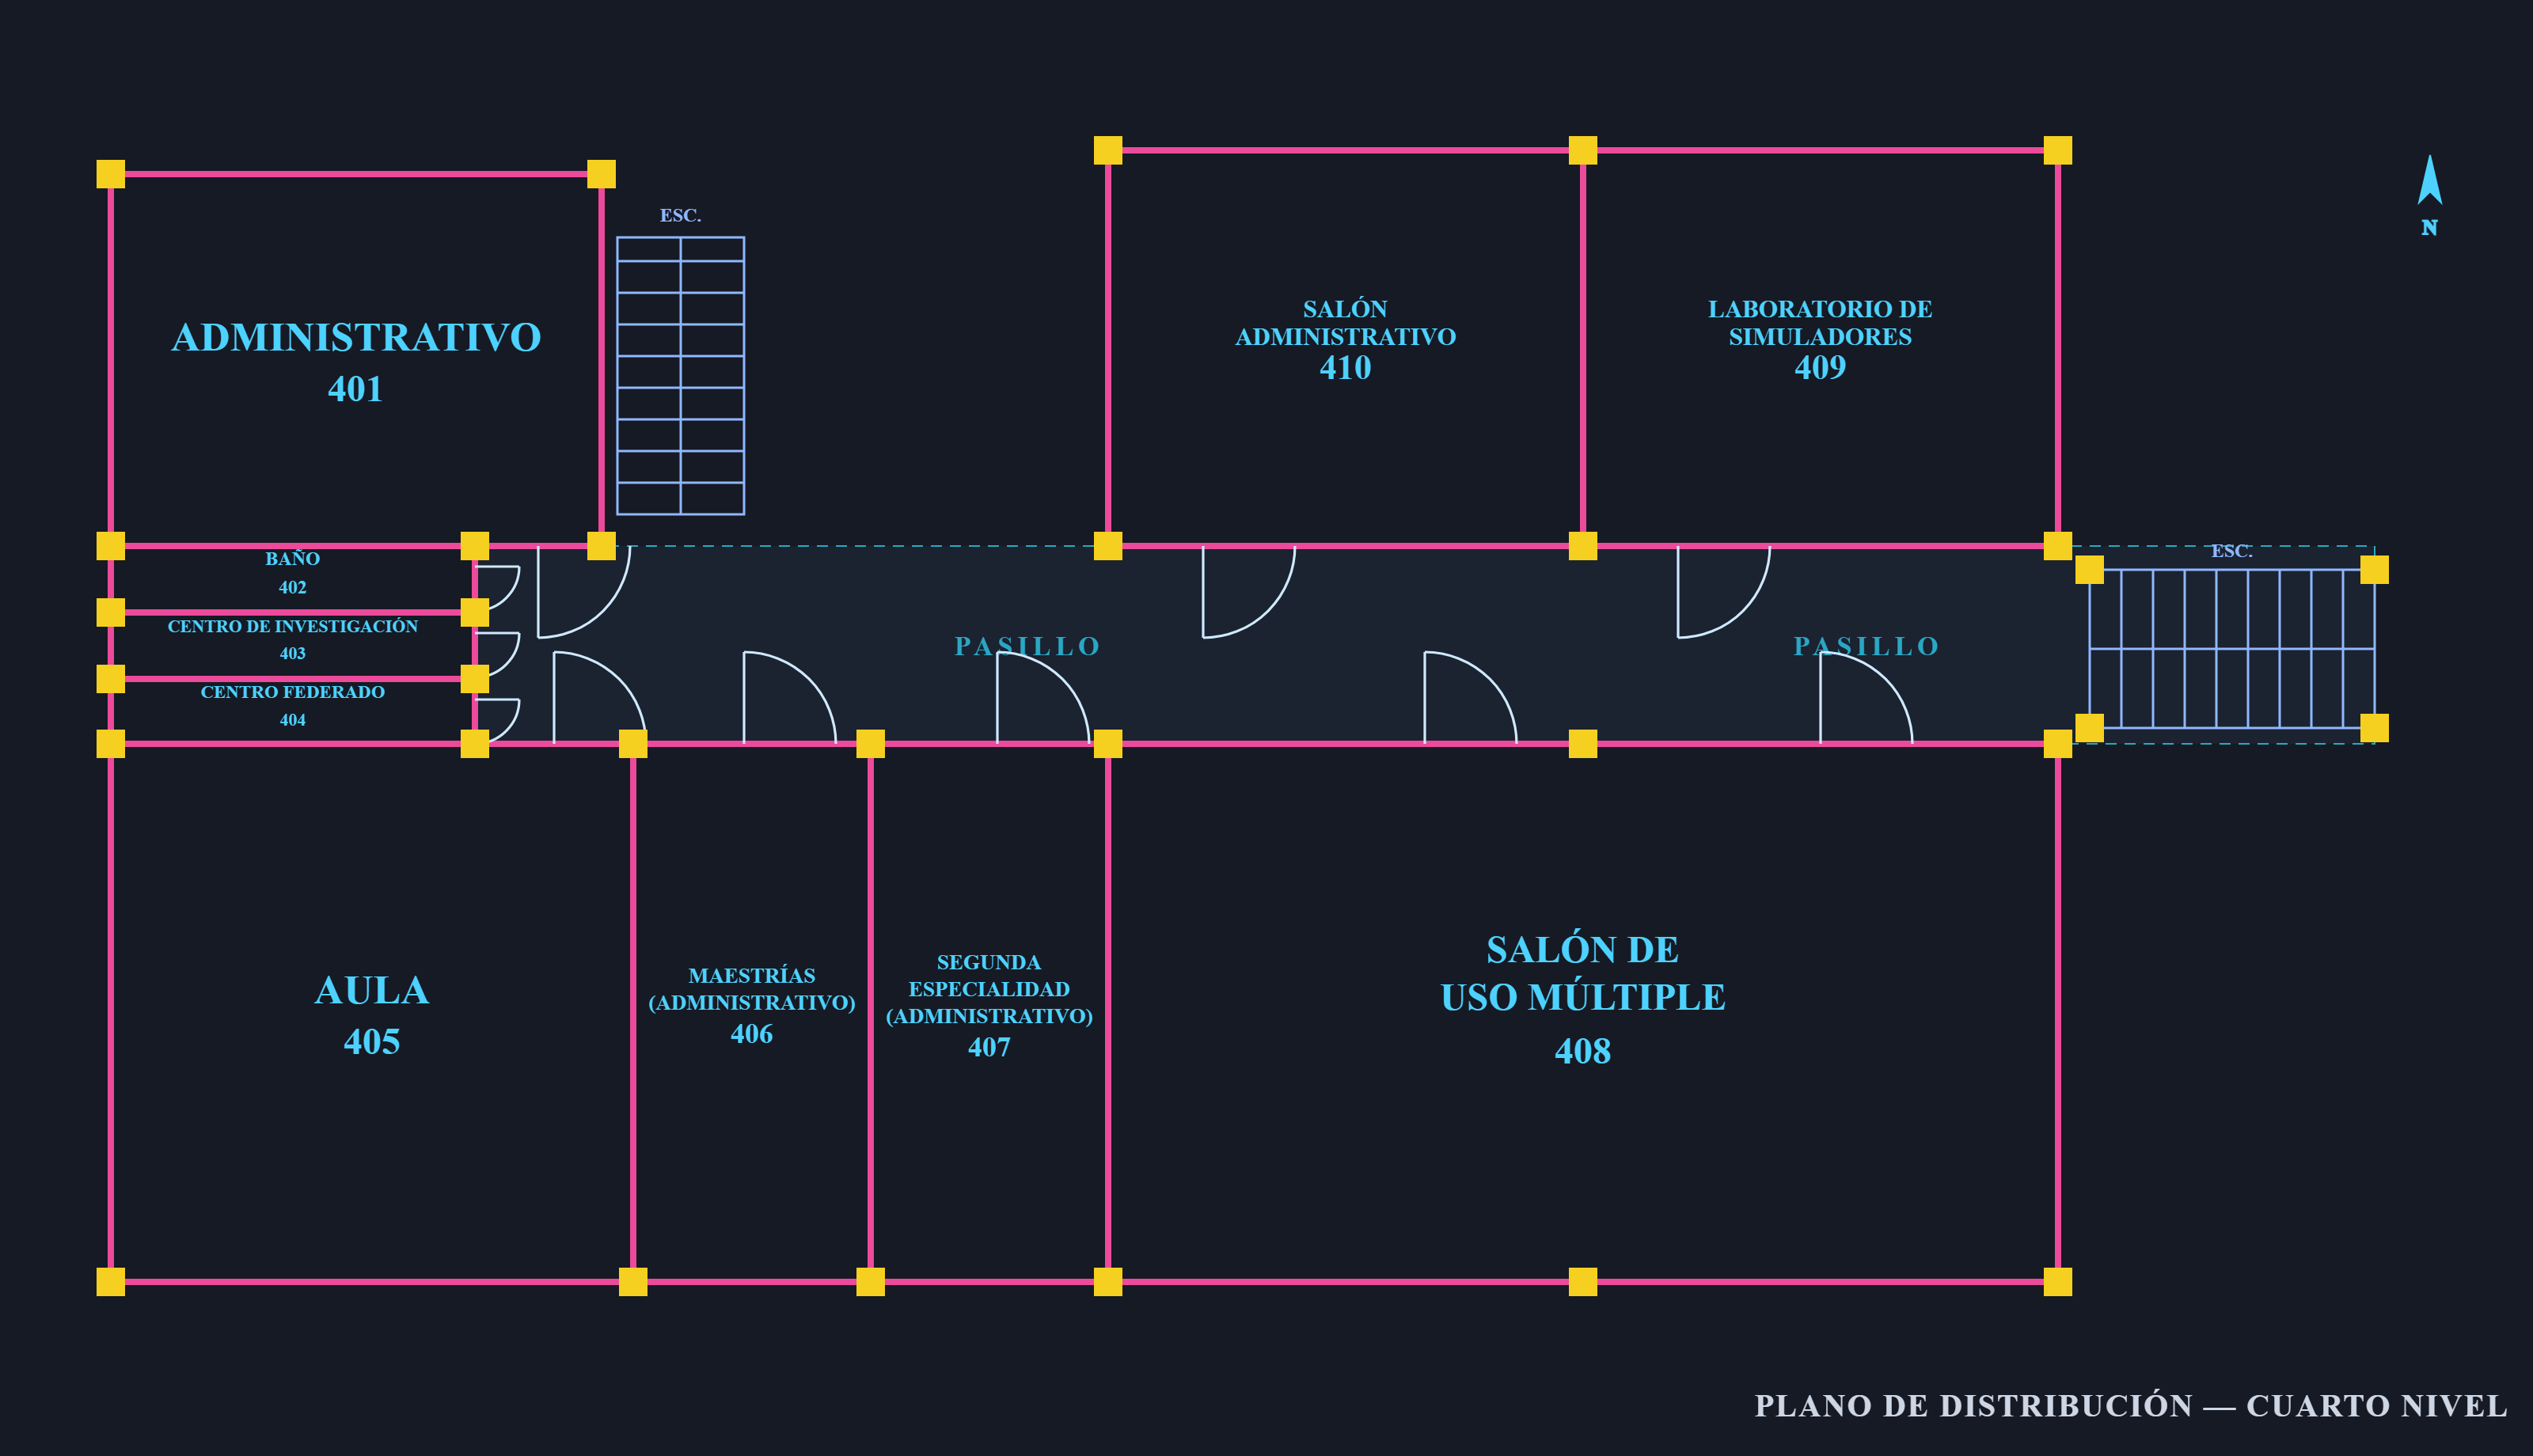
\includegraphics[width=0.97\textwidth]{images/imagenes/plano_cuarto_nivel1.png}
    \caption{Plano del cuarto nivel con puntos de red G09-D14 a G09-D29 y ubicación del Gabinete G09 (MDF). Esc.\ 1:100.}
    \label{fig:plano_cuarto_nivel}
\end{figure}

\subsection{Resumen Consolidado por Nivel}
A fin de inventariar la infraestructura pasiva y asegurar la consistencia del proyecto, se presenta la matriz de distribución física de los cables que bajan directamente hacia el Rack G09 en el segundo piso. Esta distribución considera una arquitectura de 7 a 8 ambientes por planta, integrando datos fijos, Wi-Fi y seguridad por video vigilancia (CCTV):

\begin{table}[H]
\centering
\caption{Resumen consolidado de infraestructura de cableado horizontal.}
\small
\begin{tabular}{lcccc}
\hline
\textbf{Nivel del Edificio} & \textbf{Datos (D)} & \textbf{Wi-Fi (W)} & \textbf{CCTV (C)} & \textbf{Total Enlaces} \\
\hline
Primer Nivel (Administración) & 10 & 2 & 2 & 14 \\
Segundo Nivel (Cómputo / Aulas) & 19 & 2 & 2 & 23 \\
Tercer Nivel (Laboratorios / Aulas) & 8 & 2 & 2 & 12 \\
Cuarto Nivel (Auditorio / Aulas) & 8 & 3 & 2 & 13 \\
\hline
\textbf{Total General de Nodos} & \textbf{45} & \textbf{9} & \textbf{8} & \textbf{62 puntos de red} \\
\hline
\end{tabular}
\end{table}

\subsection{Canalizaciones y Criterios de Tendido}
El despliegue físico del cableado horizontal se regirá bajo las pautas de las normas ANSI/TIA-569-D y ANSI/TIA-568-C.2, adaptadas a un entorno universitario:
\begin{itemize}[label=$\bullet$,leftmargin=1.4em]
    \item \textbf{Longitud Máxima de Canal:} Ningún cable horizontal de cobre excederá los 90 metros de distancia lineal desde el jack de la pared hasta el Patch Panel del segundo piso, garantizando la integridad de la transmisión Gigabit.
    \item \textbf{Factor de Ocupación:} El dimensionamiento de las canaletas de PVC adosadas y de las tuberías de paso respetará un máximo del 40\,\% de su capacidad transversal útil, permitiendo una ventilación adecuada y holgura para futuras expansiones.
    \item \textbf{Segregación de Servicios:} Se mantendrá una separation física mínima de 150\,mm respecto a cualquier conductor de energía eléctrica en trayectorias paralelas, mitigando riesgos de inducción electromagnética sobre la red de datos.
\end{itemize}

\section{Plano de Racks, Patch Panels y Salas de Telecomunicaciones}
\label{sec:plano_racks}

Las salas de telecomunicaciones (TR, según \mbox{ANSI/TIA-569-D}) son espacios dedicados a equipos activos, patch panels, UPS y demás componentes del cableado estructurado. Su diseño incide directamente en la confiabilidad y escalabilidad de la red.

\subsection{MDF --- Gabinete G09}
Al centralizar toda la red del pabellón en un único Rack Principal (MDF) ubicado en el segundo piso, se elimina la necesidad de backbones verticales de fibra interna, abaratando costos de fusiones y módulos ópticos.
El gabinete aloja la terminación del cableado horizontal de cobre y los equipos activos principales. A modo referencial se consideran marcas reconocidas en el mercado de telecomunicaciones:

\begin{table}[H]
\centering
\caption{Características físicas y de hardware del Gabinete G09.}
\begin{tabular}{ll}
\hline
\textbf{Parámetro del Sistema} & \textbf{Especificación de Ingeniería} \\
\hline
Tipo de Estructura & Gabinete cerrado de 19'' con paneles desmontables y llave \\
Altura Útil & 42U (espacio suficiente para crecimiento modular de la facultad) \\
Paneles de Parcheo & 3 Patch Panels Cat.\,6A de 24 puertos (72 puertos totales) \\
Equipamiento Activo & 2 Switches de 48 puertos PoE+ (96 puertos para 62 nodos) \\
Respaldo de Energía & 1 UPS Online de Doble Conversión de 1500\,VA \\
Gestión Térmica & Ventilación forzada superior con termostato integrado \\
\hline
\end{tabular}
\end{table}

\begin{figure}[H]
    \centering
    \imgpend[0.75\textwidth]{Elevaci\'{o}n frontal del rack (pendiente)}
    \caption{Diagrama de elevación frontal del rack en 2D que ilustra la distribución por unidades (U), mostrando de arriba a abajo la alternancia entre organizadores de cable horizontales, los tres Patch Panels, los dos switches y, en la base, la UPS.}
    \label{fig:elevacion_rack_mdf}
\end{figure}

\section{Plano de Backbone}
\label{sec:plano_backbone}

\begin{figure}[H]
    \centering
    \imgpend[0.85\textwidth]{Diagrama de backbone del campus (pendiente)}
    \caption{Diagrama esquemático de bloques que representa la interconexión externa del edificio de Enfermería, mediante un cable de fibra óptica monomodo (OS2) que llega desde el centro de distribución general (DTIC-UNSAAC) hasta el panel de fibra (ODF) del Rack G09.}
    \label{fig:diagrama_backbone}
\end{figure}

\section{Detalles Constructivos de Ductos, Bandejas y Registros}
\label{sec:detalles_constructivos}

\begin{figure}[H]
    \centering
    \imgpend[0.85\textwidth]{Detalles constructivos de ductos (pendiente)}
    \caption{Dibujos técnicos de corte transversal que especifican las dimensiones de las canaletas de PVC, el anclaje de soportes en el techo para los tramos principales y las cajas de registro de paso. Conviene mostrar el cable ocupando como máximo el 40\,\% de la sección.}
    \label{fig:detalles_constructivos_ductos}
\end{figure}

\section{Diagrama de Puesta a Tierra}
\label{sec:puesta_a_tierra}

Un sistema de puesta a tierra deficiente genera interferencia electromagnética, ruido y daño por sobretensiones en los equipos de red. Por ello, el diseño sigue la norma \textbf{\mbox{ANSI/TIA-607-B}}, que establece los requisitos de equipotencialización (bonding) para infraestructura de telecomunicaciones.

\begin{figure}[H]
    \centering
    \imgpend[0.85\textwidth]{Diagrama de puesta a tierra (pendiente)}
    \caption{Esquema unifilar del sistema de puesta a tierra, detallando la conexión del chasis del Rack G09 hacia la barra de cobre de telecomunicaciones (TGB) mediante un conductor verde normado, y de allí hacia el pozo a tierra. Anotar el valor objetivo $\le 5\,\Omega$.}
    \label{fig:diagrama_puesta_tierra}
\end{figure}

\section{Infraestructura de Soporte para Cobertura Inalámbrica}
\label{sec:cobertura_wifi}
Dado que el proyecto se centra en la capa física (cableado), la planificación inalámbrica se limita a garantizar la \textbf{infraestructura de cable} necesaria para los Access Points. Cada AP se alimenta y conecta mediante un único enlace de cobre Cat.\,6A con PoE+ desde el switch del Rack G09, sin requerir tomacorrientes locales.

La distribución de los 9 Access Points se calcula en función del aforo y la naturaleza de cada piso:
\begin{itemize}[label=$\bullet$,leftmargin=1.4em]
    \item \textbf{Piso 1 (2 APs):} Ubicados en el pasillo administrativo y la zona abierta de la Sala de Lectura.
    \item \textbf{Piso 2 (2 APs):} Dispuestos en las aulas teóricas colindantes y el Centro de Cómputo.
    \item \textbf{Piso 3 (2 APs):} Dedicados a los salones de práctica y laboratorios de simulación de Enfermería.
    \item \textbf{Piso 4 (3 APs):} Dos puntos para las aulas de las alas este y oeste, y un punto de alta densidad para el Auditorio Principal.
\end{itemize}

\begin{figure}[H]
    \centering
    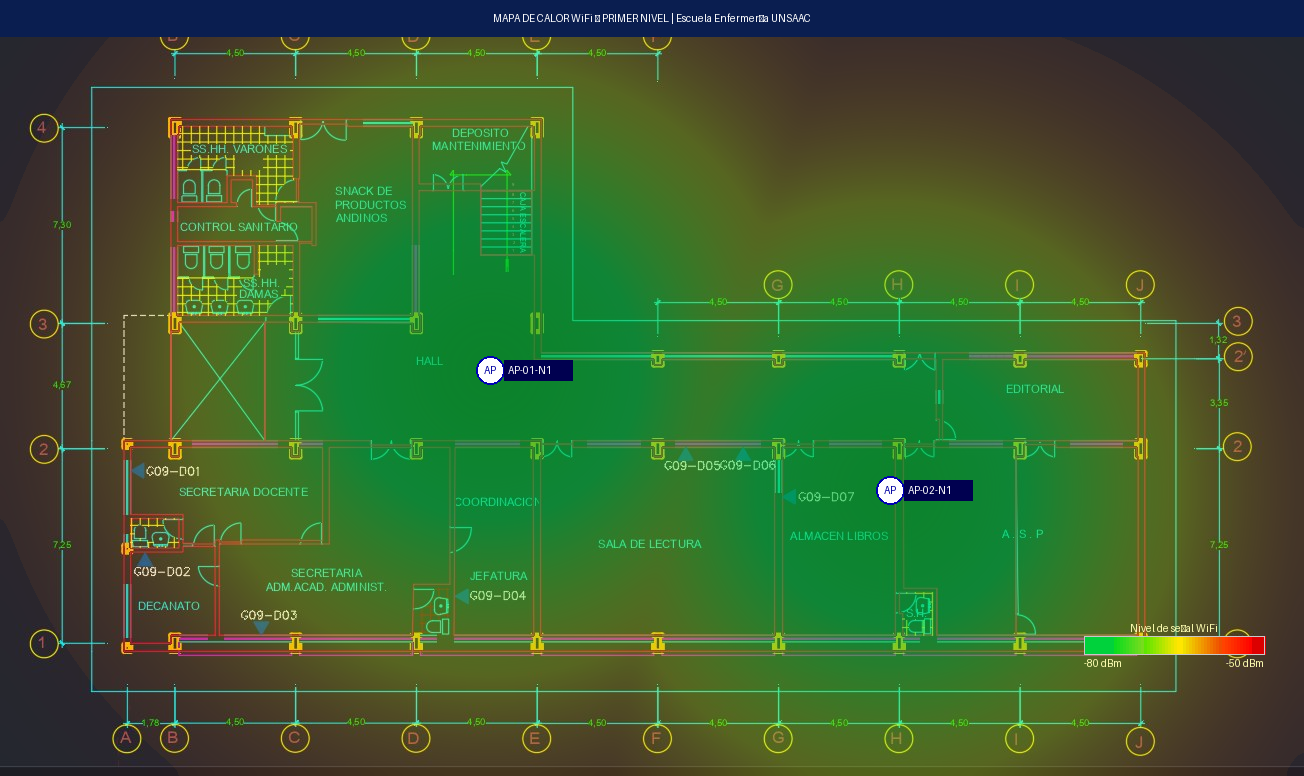
\includegraphics[width=0.95\textwidth]{images/imagenes/mapa_calor_primer_nivel.png}
    \caption{Mapa de calor WiFi — Primer nivel. AP-01-N1 en hall central y AP-02-N1 en sala de lectura. Escala cromática: verde ($\geq -50$\,dBm, excelente) a rojo (zona muerta, $< -85$\,dBm).}
    \label{fig:mapa_calor_1}
\end{figure}

\begin{figure}[H]
    \centering
    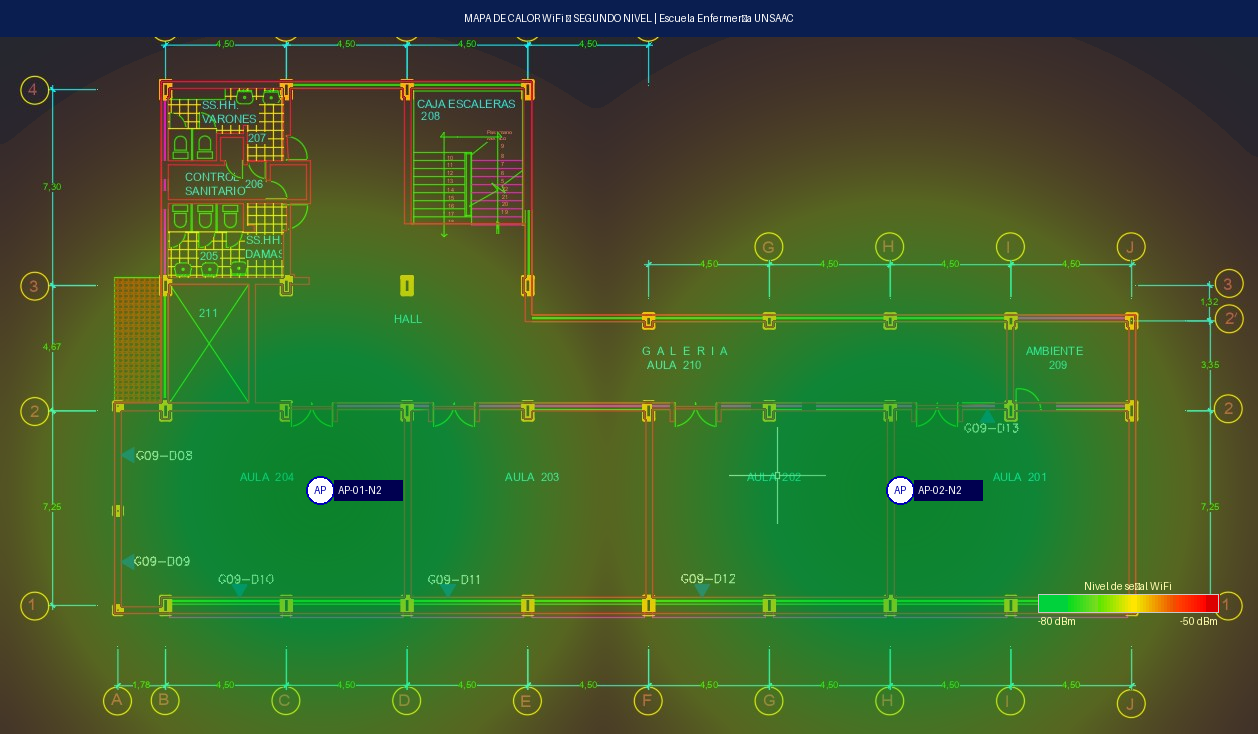
\includegraphics[width=0.95\textwidth]{images/imagenes/mapa_calor_segundo_nivel.png}
    \caption{Mapa de calor WiFi — Segundo nivel. AP-01-N2 cubre aulas 203/204 y AP-02-N2 cubre aulas 201/202. Se aprecia el solapamiento de celdas (15--20\%) necesario para roaming continuo.}
    \label{fig:mapa_calor_2}
\end{figure}

\begin{figure}[H]
    \centering
    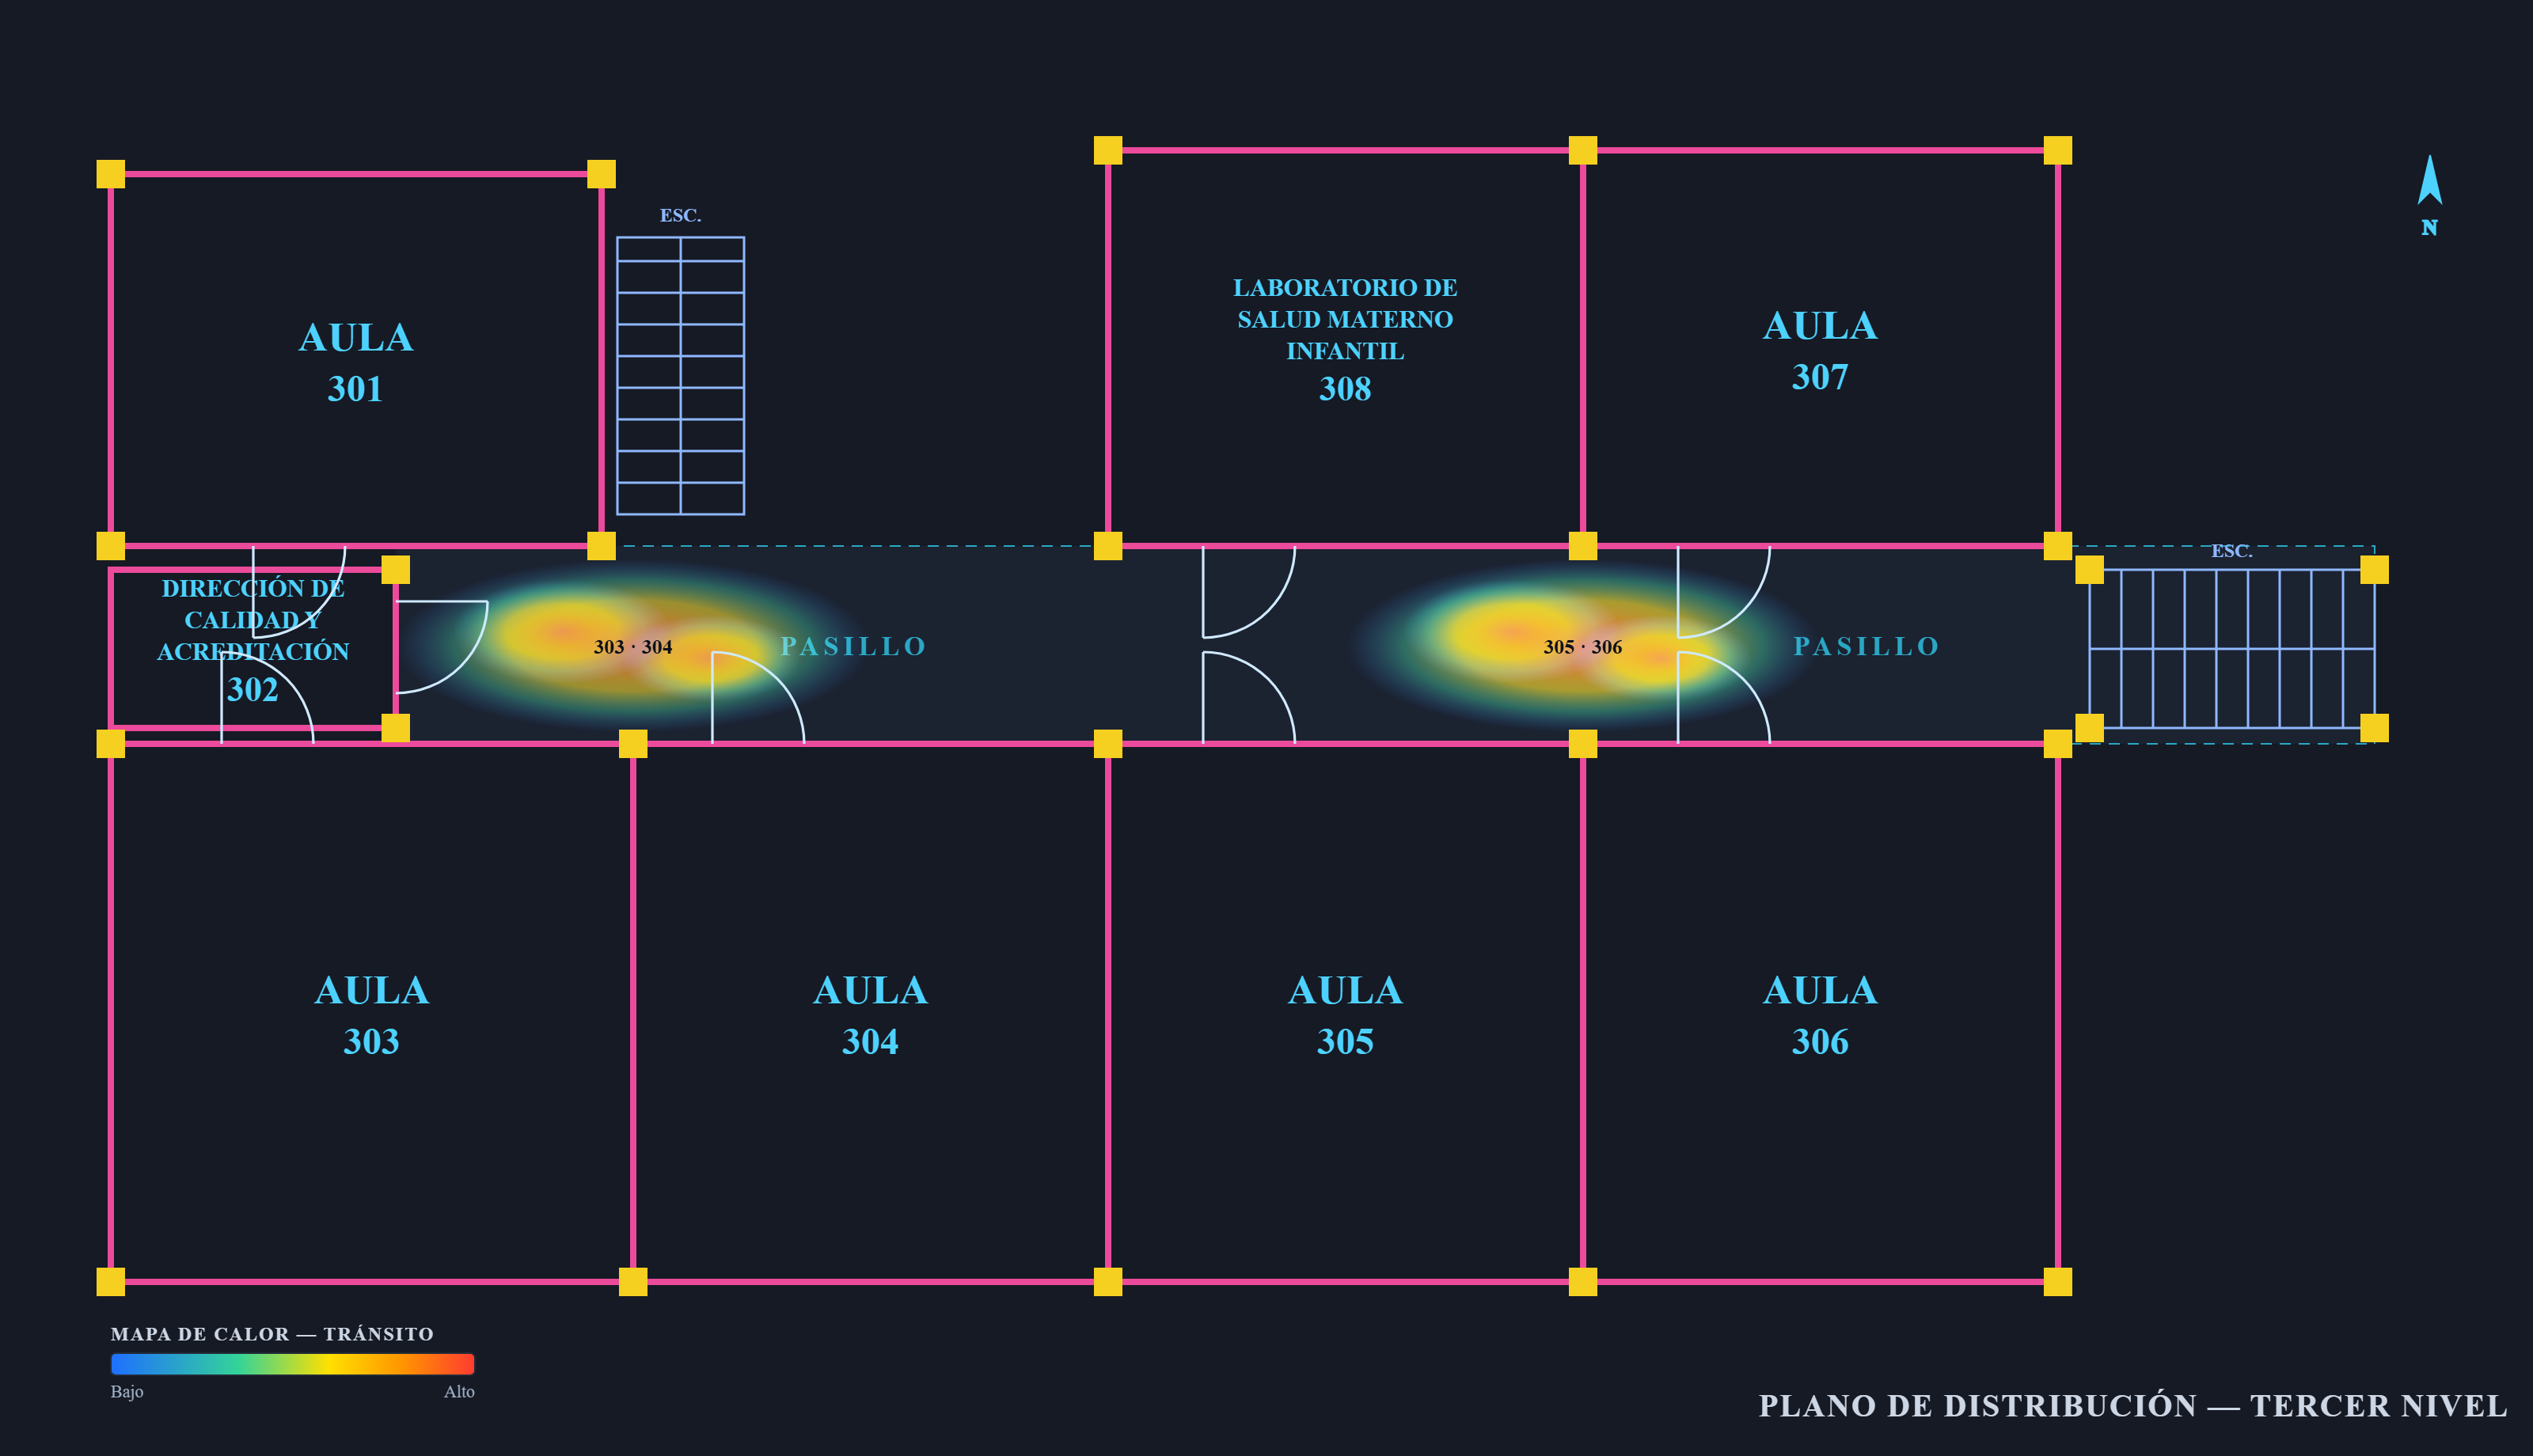
\includegraphics[width=0.95\textwidth]{images/imagenes/mapa_calor_tercer_nivel.png}
    \caption{Mapa de calor WiFi — Tercer nivel. AP-01-N3 y AP-02-N3 cubren los ambientes de trabajo; AP-03-N3 brinda cobertura dedicada en el Salón de Grados. La sala de telecomunicaciones (Gabinete G09) queda excluida por ser de acceso restringido.}
    \label{fig:mapa_calor_3}
\end{figure}

\begin{figure}[H]
    \centering
    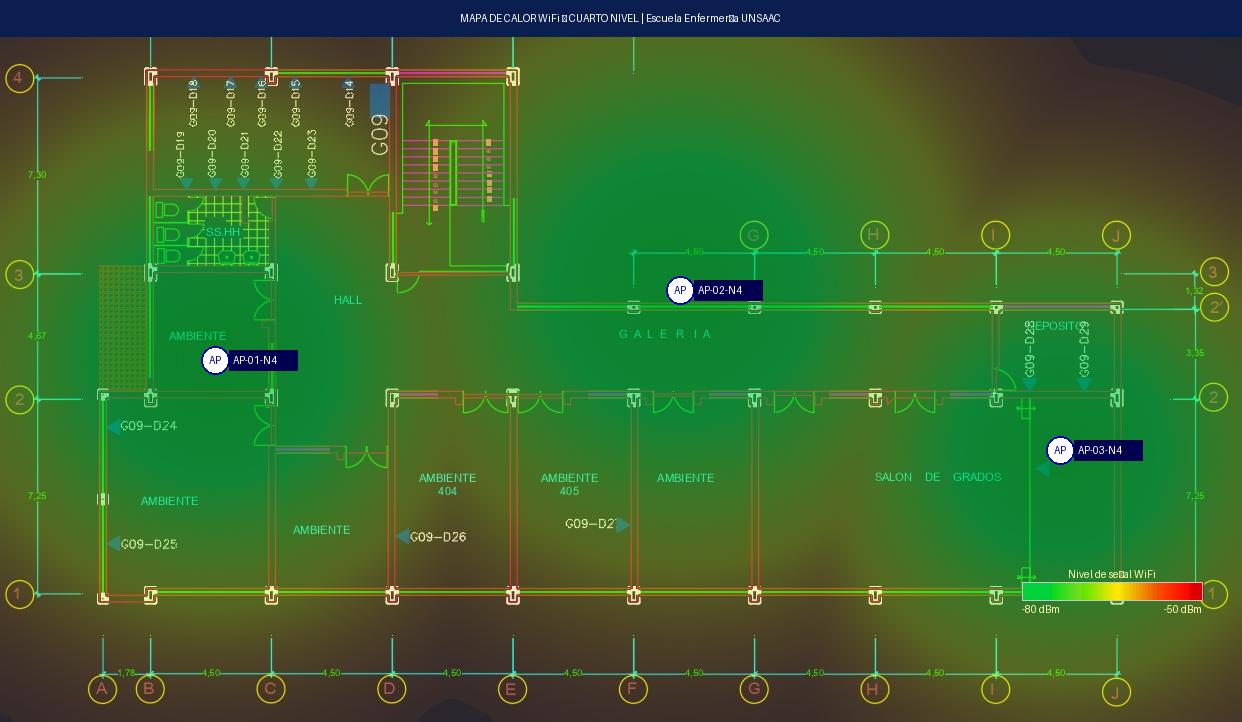
\includegraphics[width=0.95\textwidth]{images/imagenes/mapa_calor_cuarto_nivel.png}
    \caption{Mapa de calor WiFi — Cuarto nivel. AP-01-N4 y AP-02-N4 cubren los ambientes de trabajo; AP-03-N4 brinda cobertura dedicada en el Salón de Grados. La sala de telecomunicaciones (Gabinete G09) queda excluida por ser de acceso restringido.}
    \label{fig:mapa_calor_4}
\end{figure}

\section{Seguridad Física de Telecomunicaciones}
\label{sec:seguridad_fisica}
El resguardo físico de la red es crítico al centralizarse en un solo nodo. Al estar ubicado el Rack G09 dentro del Centro de Cómputo del segundo piso, se beneficia de las medidas existentes del ambiente: acceso restringido mediante cerradura de seguridad, llaves térmicas eléctricas exclusivas para el laboratorio y supervisión constante por parte del personal de la escuela, cumpliendo con los lineamientos básicos de protección de infraestructura universitaria.